\normaltrue \difficilefalse \tdifficilefalse
\correctionfalse

%\UPSTIidClasse{11} % 11 sup, 12 spé
%\newcommand{\UPSTIidClasse}{11}

\exer{Identification temporelle $\star$ \label{B2:06:502}}
\setcounter{numques}{0}
\UPSTIcompetence[2]{B2-06}
\index{Compétence B2-06}
\index{Identification}
\index{Identification temporelle}
\index{Ordre 1}
\index{Ordre 2}
\ifcorrection
\else
\textbf{Pas de corrigé pour cet exercice.}
\fi


\ifprof 
\else
Soit la réponse à un échelon.
\begin{center}
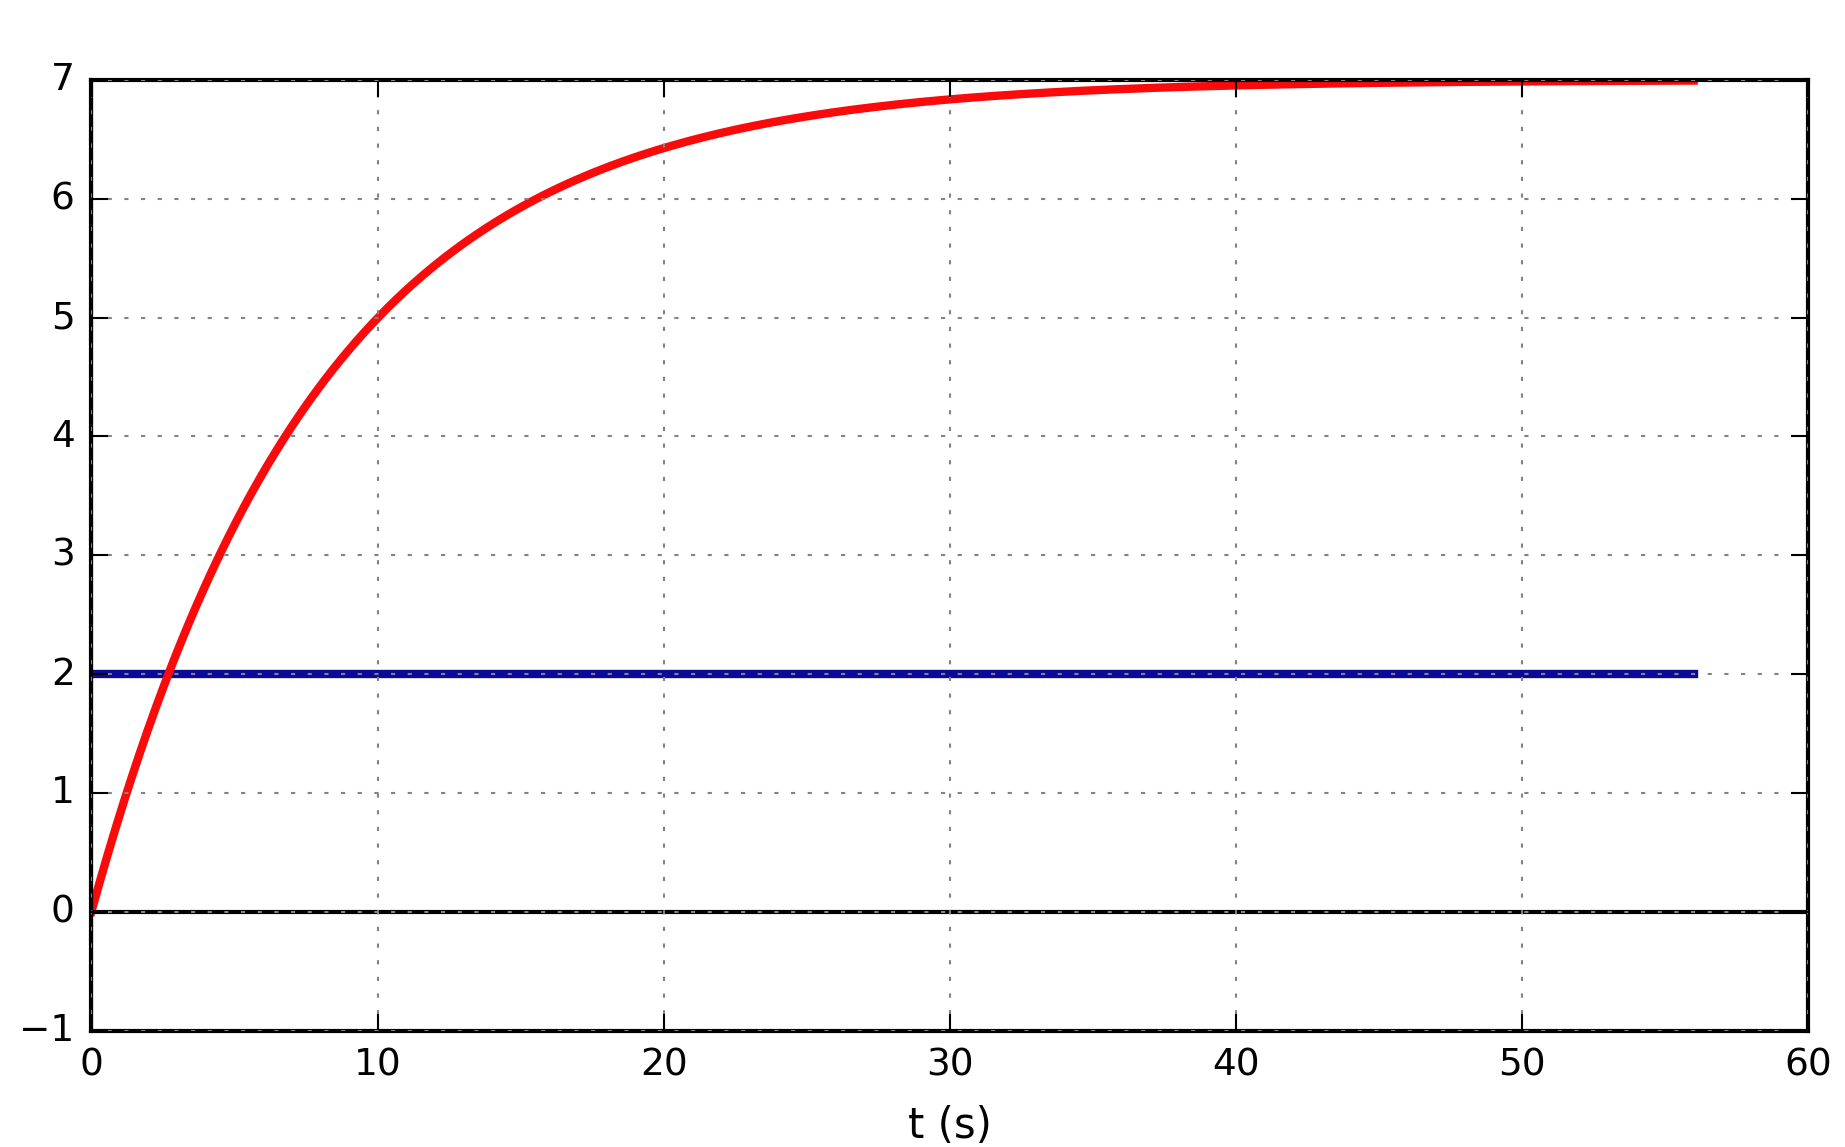
\includegraphics[width=.9\linewidth]{502_01}
\end{center}
\fi

\question{Déterminer la fonction de transfert du système.}
\ifprof
%\begin{figure}[H]
%\centering
%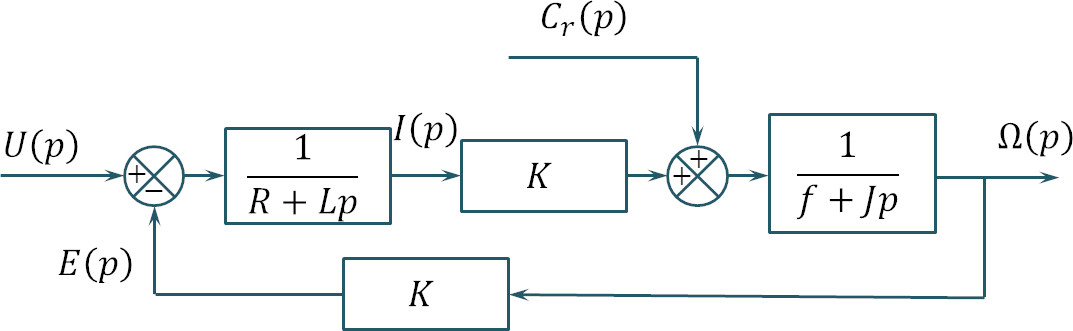
\includegraphics[width=\linewidth]{51_01_c}
%\caption{Évolution du couple utile en fonction de la vitesse de rotation pour des
%fréquences de commande de \SI{90}{Hz} à \SI{110}{Hz}. \label{fig_50_04}}
%\end{figure}
\else
\fi



\ifprof 
\else
Soit la réponse à un échelon d'amplitude 2,5.

\begin{center}
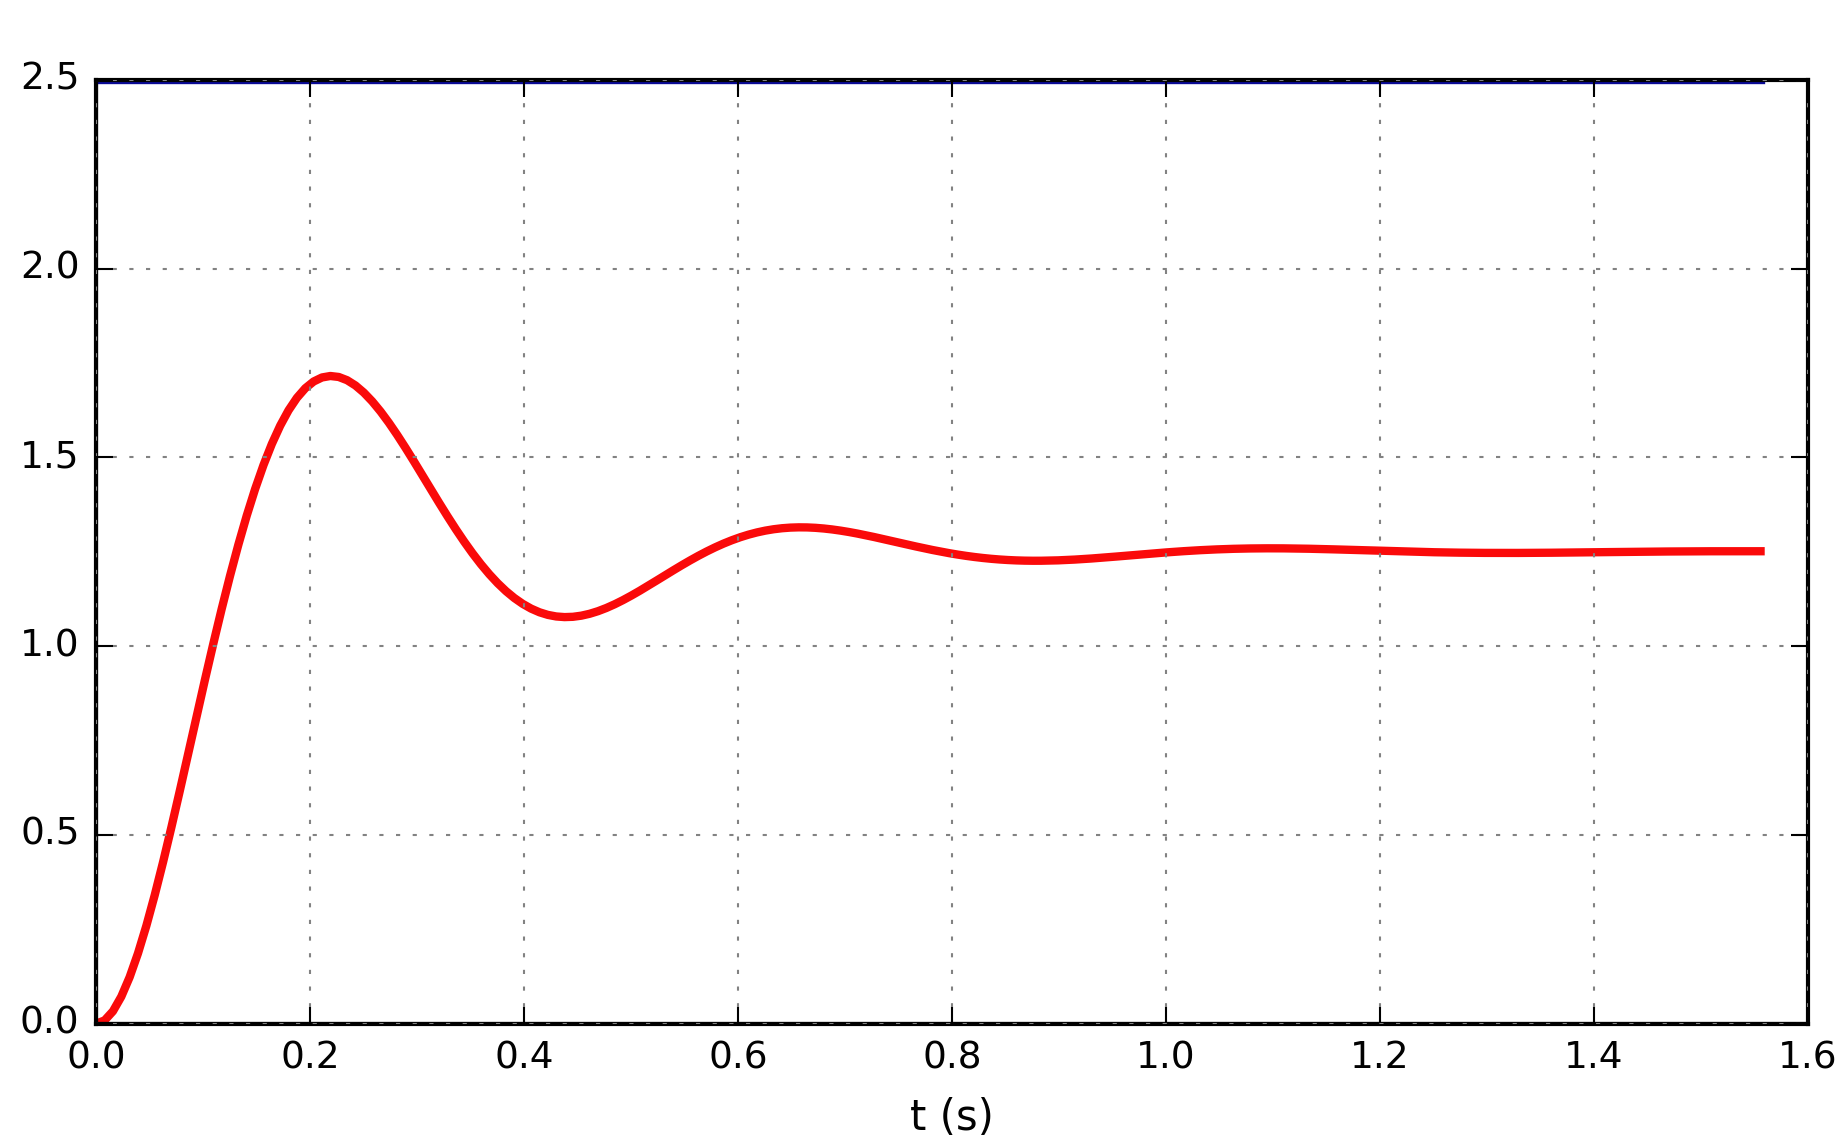
\includegraphics[width=.9\linewidth]{502_02}
\end{center}
\fi

\question{Déterminer la fonction de transfert du système.}
\ifprof
%\begin{figure}[H]
%\centering
%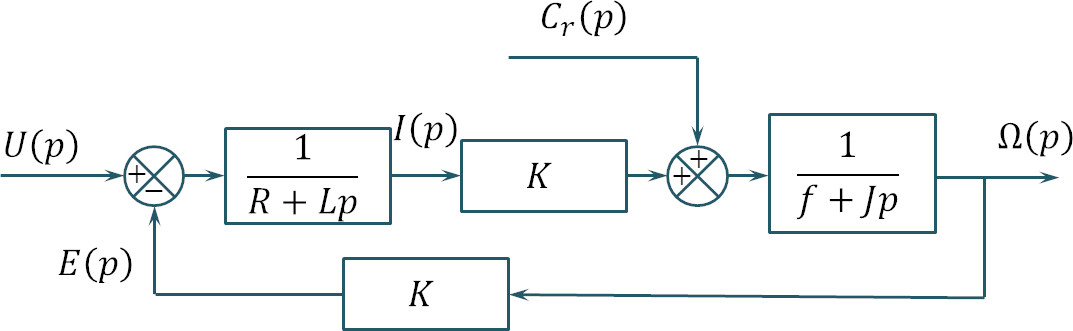
\includegraphics[width=\linewidth]{51_01_c}
%\caption{Évolution du couple utile en fonction de la vitesse de rotation pour des
%fréquences de commande de \SI{90}{Hz} à \SI{110}{Hz}. \label{fig_50_04}}
%\end{figure}
\else
\fi



\ifprof
\else
\begin{flushright}
\footnotesize{Corrigé  voir \ref{B2:06:502}.}
\end{flushright}%
\fi